\chapter{Introduction}
\label{ch:introduction}

% ============================================================
\section{Motivation}
\label{sec:intro:motivation}
% ============================================================

This thesis addresses a weakly supervised classification problem at
the intersection of computer vision, fuzzy logic, and biomedical
informatics.
The input is a gigapixel whole-slide image (WSI) of a tissue
biopsy---typically $10^9$--$10^{10}$ pixels, comparable in file size
to a feature film---and the output is a binary prediction for each of
several target genes: \emph{mutated} or \emph{wild-type} (normal).
The only supervision available is a single patient-level label per
gene; no annotation indicates \emph{which} regions of the image carry
the mutation signal.
This is the canonical multiple-instance learning (MIL) setting,
where each image is a ``bag'' of thousands of ``instances'' (tiles)
and only the bag-level label is known.

The application domain is lung adenocarcinoma
(LUAD)~\cite{sung2021global}, the most common subtype of lung
cancer.
In clinical oncology, knowing which genes are mutated determines
which drugs a patient can receive: for example, patients with
\emph{EGFR} mutations benefit from targeted inhibitors that are
ineffective for wild-type patients~\cite{herbst2018lung}.
The gold standard for mutation detection is DNA sequencing, which
requires specialised laboratory infrastructure, trained personnel,
and significant turnaround
times~\cite{vanderlaan2018molecular}---a critical delay during which
patients cannot receive optimal treatment.
In resource-limited settings, sequencing may not be available at
all~\cite{sung2021global}.

\emph{Computational pathology} offers an alternative: since every
patient already has a stained tissue slide examined by a pathologist,
a model that can ``read'' mutation signals from the slide image could
provide a rapid preliminary prediction without additional laboratory
procedures.
Deep learning methods have demonstrated that this is
feasible~\cite{coudray2018classification, kather2020pancancer,
saldanha2023npj}, but existing approaches exhibit two fundamental
limitations that motivate this thesis:

\paragraph{Limitation 1: The interpretability gap.}
End-to-end convolutional neural networks (e.g., Inception-v3~\cite{coudray2018classification}) and large-scale foundation models (e.g., CHIEF~\cite{wang2024chief}, GigaPath~\cite{xu2024gigapath}) learn internal feature representations that do not correspond to any named histopathological entity.  When such a model predicts ``TP53 mutated, confidence 0.83,'' no human-readable explanation is available.  A pathologist cannot verify, critique or contextualise the prediction.  This severely limits clinical adoption, as clinical decision-support systems require \emph{actionable interpretability}---not merely a confidence score, but a reasoning pathway expressed in the language of the domain~\cite{holzinger2019causability}.

\paragraph{Limitation 2: The data-scale barrier.}

Recent state-of-the-art results have been achieved with proprietary
multicentric datasets of thousands of patients:
DeepGEM~\cite{zhao2025deepgem} used 3{,}637 patients from 16 Chinese
hospitals; EAGLE~\cite{campanella2025eagle} used 8{,}461 slides with
Microsoft Research resources; CHIEF was pretrained on 60{,}530 whole-slide images and GigaPath on
1.3 billion pathology tiles from 171{,}189 slides, respectively.
These resources are categorically unavailable to the vast majority of
academic research groups.
The largest publicly accessible LUAD cohort with paired WSIs and mutation
annotations is The Cancer Genome Atlas (TCGA), comprising approximately
668 patients (687 slides)~\cite{tcga2014luad}---two orders ofmagnitude smaller than these industrial-scale datasets.\footnote{The
TCGA-LUAD project on the GDC has expanded since its original 2014 release.
This thesis uses 687 slides from 668 unique patients; 19 patients
contributed more than one slide.
The commonly cited figure of $\sim$557 refers to the case count in the
original TCGA publication~\cite{tcga2014luad}.}Methods that require massive data to achieve competitive performance are
therefore not directly applicable in data-scarce research environments.
\paragraph{The opportunity: domain knowledge as a computational prior.}
LUAD is classified by the World Health Organisation (WHO) into five predominant growth patterns---lepidic, acinar, papillary, micropapillary, and solid---each with documented statistical associations with specific molecular subtypes~\cite{travis2011iaslc, tsao2015subtype}.  This thesis adopts the six ANORAK-annotated growth patterns (the five WHO patterns plus cribriform) as domain knowledge that has never been explicitly incorporated as a \emph{structured computational prior} into modern mutation prediction pipelines.  This thesis explores whether doing so can compensate for data scarcity while simultaneously providing the interpretable reasoning pathway that end-to-end models lack.

% ============================================================
\section{Hypothesis}
\label{sec:intro:hypothesis}
% ============================================================

This thesis investigates the following central hypothesis:

\begin{quote}
\textbf{H:} \emph{Structured domain knowledge---specifically,
expert-defined histological growth patterns encoded through fuzzy set
theory---can be injected into a deep learning mutation prediction
pipeline to simultaneously
(a)~achieve competitive predictive performance under data scarcity
($<$700 public slides), and
(b)~render the resulting predictions \textbf{interpretable} through
a multi-level, clinically verifiable inspection framework---and,
through that framework, \textbf{explainable} via knowledge-graph--grounded
natural-language rationales---to a degree that no end-to-end black-box
approach offers.}
\end{quote}

The two italicised terms in clause~(b) carry the technical
meanings established in
Section~\ref{sec:bg:xai:definitions}---\emph{interpretability}
as a structural property of the model (the six-level inspection
framework, the intrinsic Choquet Shapley values, and the
Conclusive/Inconclusive cohort flag) and \emph{explainability}
as the post-hoc, knowledge-graph--grounded natural-language layer
built on top of it---and they are claimed at different evidence
levels: the interpretability claim is empirically tested in
Chapter~\ref{ch:evaluation}; the explainability layer is
implemented and inspected qualitatively, but its formal
evaluation (faithfulness audit, knowledge-graph correctness, and
reader study) is reserved for future work
(Section~\ref{sec:disc:future}).

The hypothesis is \emph{gene-conditional} and
\emph{aggregator-conditional} rather than all-or-nothing: whether
fuzzy pattern knowledge yields a predictive gain for a given gene
depends jointly on (a) whether the discriminative signal for that
gene admits a representation within the ANORAK 6-pattern ontology,
and (b) whether the downstream aggregator can read that
representation.
Each gene in the panel therefore constitutes an independent test of
\textbf{H}, and the verdict on \textbf{H} is the conjunction of the
per-gene verdicts together with the system-level instrumentation
test below.

Operationally, the hypothesis is \emph{falsifiable} along three
independent axes.
It would be rejected if
(i)~pattern-informed models systematically degraded predictive
performance below embedding-only baselines for \emph{every} gene in
the target panel;
(ii)~no aggregation mechanism in the candidate space (additive
concatenation, learned attention, or fuzzy Choquet integral) could
exploit the pattern channel to outperform the embedding-only
baseline for \emph{any} gene;
or (iii)~the proposed pipeline could not be \emph{instrumented} to
produce the six interpretability layers end to end, or the
resulting explanations could not be grounded in provenance-tagged
ontology IRIs.
Genes for which no aggregator within the ANORAK simplex recovers a
discriminative signal are themselves a finding to be characterised
under RQ2(ii)---the \emph{coverage} limit of the pattern
ontology---rather than evidence against the hypothesis as a whole.
The seven research questions below operationalise this hypothesis
into testable sub-questions.

% ============================================================
\section{Research Questions}
\label{sec:intro:rq}
% ============================================================

Guided by the design science research (DSR) paradigm~\cite{hevner2004design, peffers2007dsrm}, which focuses on the construction and evaluation of artefacts that address identified problems, this thesis formulates the following research questions from a computer science and engineering perspective.
Each RQ addresses a specific aspect of the central hypothesis (Section~\ref{sec:intro:hypothesis}):

\begin{description}
    \item[\textbf{RQ1} (Fuzzy representation learning).]  \emph{How can fuzzy set theory be integrated into angular margin loss functions to produce an adaptive, per-sample margin modulation mechanism for histopathological pattern classification, and does the resulting loss function outperform fixed-margin baselines under conditions of small training sets and fuzzy inter-class boundaries?}

    \item[\textbf{RQ2} (Pattern-informed multiple-instance learning).]
    This question is decomposed into two complementary sub-questions:
    \begin{description}
        \item[\textbf{RQ2(i)}.]
        \emph{Can the explicit injection of fuzzy histological pattern
        probabilities---derived from a validated pattern classifier---as
        structured features into an attention-based MIL aggregator
        improve or preserve mutation prediction performance relative to
        using visual embeddings alone, thereby providing an interpretable
        morphological reasoning channel?}
        \item[\textbf{RQ2(ii)}.]
        \emph{For the genes where pattern injection does not improve
        performance, which mutations have no exploitable morphological
        footprint within the ANORAK 6-pattern ontology, and what
        mechanisms account for these failures?}
    \end{description}
    The two parts together frame RQ2 as a question about both the
    \emph{utility} and the \emph{coverage} of the pattern channel.

    \item[\textbf{RQ3} (Fuzzy aggregation for mutation prediction).]  \emph{Does a fuzzy Choquet integral aggregation module, which models supra-additive interactions among histological pattern memberships through a learned fuzzy measure, capture biologically meaningful inter-pattern dependencies that standard attention pooling mechanisms miss?}

    \item[\textbf{RQ4} (Clinically meaningful interpretability).]
\emph{Does the pattern-informed approach yield
\textbf{interpretability} (in the sense of
Section~\ref{sec:bg:xai:definitions})---through a six-level
inspection framework comprising spatial attention maps, pattern
overlays, SHAP decomposition, intrinsic Choquet Shapley values,
per-slide feature channel ablation, and fuzzy linguistic
labels---that a pathologist could in principle verify against the
original slide?
Do fuzzy linguistic labels computed by the system and injected
into LLM-generated rationales prevent hallucination of intensity
terms?}
RQ4 concerns the \emph{structural} interpretability of the
model and is evaluated empirically
(Chapter~\ref{ch:evaluation}); its companion question
RQ6 below concerns the \emph{post-hoc} natural-language
explanation layer.
  \item[\textbf{RQ5} (Data scarcity).]
    \emph{Does the incorporation of domain knowledge (validated histological
    patterns) via fuzzy logic provide a greater relative benefit under data
    scarcity (687 TCGA-LUAD slides) than it would under data abundance, thereby
    offering a methodological alternative to the brute-force scaling pursued
    by foundation models?}
 
    \item[\textbf{RQ6} (Ontology-grounded explainability).]
    \emph{Can the pipeline produce ontology-grounded,
    provenance-tagged natural-language case explanations
    (\textbf{explainability} in the sense of
    Section~\ref{sec:bg:xai:definitions}) that link predicted
    histological patterns, mutation hypotheses, and therapeutic
    options in a clinically auditable knowledge graph?}
    RQ6 establishes the explainability layer as a system
    capability; its formal evaluation (faithfulness audit,
    knowledge-graph correctness, and reader study) is left to
    future work and is enumerated in
    Section~\ref{sec:disc:future}.
 
    \item[\textbf{RQ7} (Knowledge graph enrichment).]
    \emph{Does the DeepSearch enrichment pipeline produce candidate new
    biomedical relations---each carrying a PMID provenance pointer and
    a type-constraint validation against NCIt/MONDO---in the executed
    run, and can these candidates be incorporated as versioned
    additions into the knowledge graph for subsequent cases, pending
    formal expert validation?}

    
\end{description}

These questions are deliberately framed from a computer science perspective.
RQ1 addresses \emph{representation learning} with fuzzy-theoretic foundations.
RQ2 addresses \emph{feature fusion} and \emph{prior knowledge
injection} in deep learning architectures, with sub-question RQ2(ii)
asking the complementary \emph{ontology-coverage} question of which
mutations have no exploitable morphological footprint.
RQ3 addresses \emph{fuzzy aggregation operators} as alternatives to neural
attention.
RQ4 addresses \emph{clinically meaningful interpretability} through spatial
attention and pattern attribution.
RQ5 addresses \emph{domain knowledge utility} under data scarcity.
RQ6 and RQ7 address \emph{ontology-grounded explainability} and
\emph{knowledge graph enrichment} as the explanation layer of the
LCHAI~v2.0 instantiation (LCHAI = \emph{Lung Cancer Histologic
Analysis with AI}, the integrative system that composes all
three artefacts and the explanation layer into a single
clinical-prototype application).
The medical domain (LUAD mutation prediction) serves as the use case in which
the artefacts are instantiated and evaluated.
% ============================================================
\section{Research Method: Fuzzy Design Science Research}
\label{sec:intro:method}
% ============================================================

This thesis follows a \emph{fuzzy design science research} (FDSR) methodology, which extends the classical DSR framework of Hevner et~al.~\cite{hevner2004design} and Peffers et~al.~\cite{peffers2007dsrm} with concepts from computational intelligence and soft computing~\cite{meier2009fuzzy}.  The FDSR cycle comprises the following eight phases, mapped to the chapters of this thesis.
The process is not strictly linear: evaluation findings feed back into artefact redesign (Ch.~6~$\to$~Ch.~4), implementation experience informs design revisions (Ch.~5~$\to$~Ch.~4), and scope is refined iteratively (Ch.~6~$\to$~Ch.~1).
The complete mapping of research questions, chapters, contributions, and publications is shown in Section~\ref{sec:intro:visual_summary} (Figure~\ref{fig:thesis_visual_summary}).

\begin{enumerate}
    \item \textbf{Problem identification and motivation} (this chapter).  The interpretability gap and data-scale barrier in mutation prediction are identified as the dual problem to be addressed.

    \item \textbf{Objectives of a solution} (this chapter, \cref{sec:intro:rq}).  Seven research questions operationalise the objectives: adaptive fuzzy loss (RQ1), pattern-informed MIL (RQ2), fuzzy aggregation (RQ3), clinically meaningful interpretability (RQ4), data scarcity (RQ5), ontology-grounded explanations (RQ6) and knowledge graph enrichment (RQ7).

    \item \textbf{Theoretical foundations} (\cref{ch:background}).  Existing theories of fuzzy sets, angular margin losses, multiple-instance learning, Choquet integrals and self-supervised pathology encoders are surveyed as the knowledge base from which artefacts are designed.

    \item \textbf{Use case definition} (\cref{ch:usecase}).  The LUAD mutation prediction problem is formalised as the application domain, including a description of the datasets, medical terminology and evaluation metrics.

    \item \textbf{Artefact design: conceptual framework} (\cref{ch:methodology}).  The three artefacts (FuzzyArcLoss V2, pattern-informed ABMIL, Fuzzy Choquet MIL) are specified at the architectural level, including their mathematical formulations and design rationale.  The multi-ontology knowledge graph and explanation layer is also designed in this chapter as a non-artifact contribution addressing RQ6 and RQ7.

    \item \textbf{Artefact implementation} (\cref{ch:implementation}).  Prototypical implementations of all artefacts are described, including training protocols, hyperparameter optimisation (Optuna), the ontology-grounded explanation layer, and the LCHAI~v2.0 clinical prototype.

    \item \textbf{Artefact evaluation} (\cref{ch:evaluation}).  Rigorous evaluation using stratified 5-fold cross-validation, statistical significance testing (paired $t$-tests, Cohen's $d$), ablation studies, comparison with published baselines, interpretability analysis with LCHAI~v2.0 pattern overlays and attention maps, and demonstration of the ontology-grounded explanation layer (RQ6, RQ7).

    \item \textbf{Communication} (\cref{ch:discussion}).  Findings are discussed in the context of the research questions, limitations are identified and an outlook for future work is provided.
\end{enumerate}


The DSR paradigm is appropriate for this thesis because the primary contributions are \emph{artefacts}---a loss function, a feature fusion architecture and an aggregation module---complemented by an ontology-grounded explanation layer and the LCHAI~v2.0 clinical prototype that instantiates all components into a functional system.  The value of these artefacts is demonstrated through their evaluation on the LUAD use case, but the artefacts themselves are general-purpose computational intelligence contributions applicable beyond cancer research.

% ============================================================
\section{Visual Summary of the Thesis}
\label{sec:intro:visual_summary}
% ============================================================

Figure~\ref{fig:thesis_visual_summary} provides a visual overview of
the thesis, mapping the seven research questions to the chapters where
they are addressed, the six contributions that result, and the three
prior publications by the author that serve as foundations for the
artefacts.

\begin{figure}[ht!]
\centering
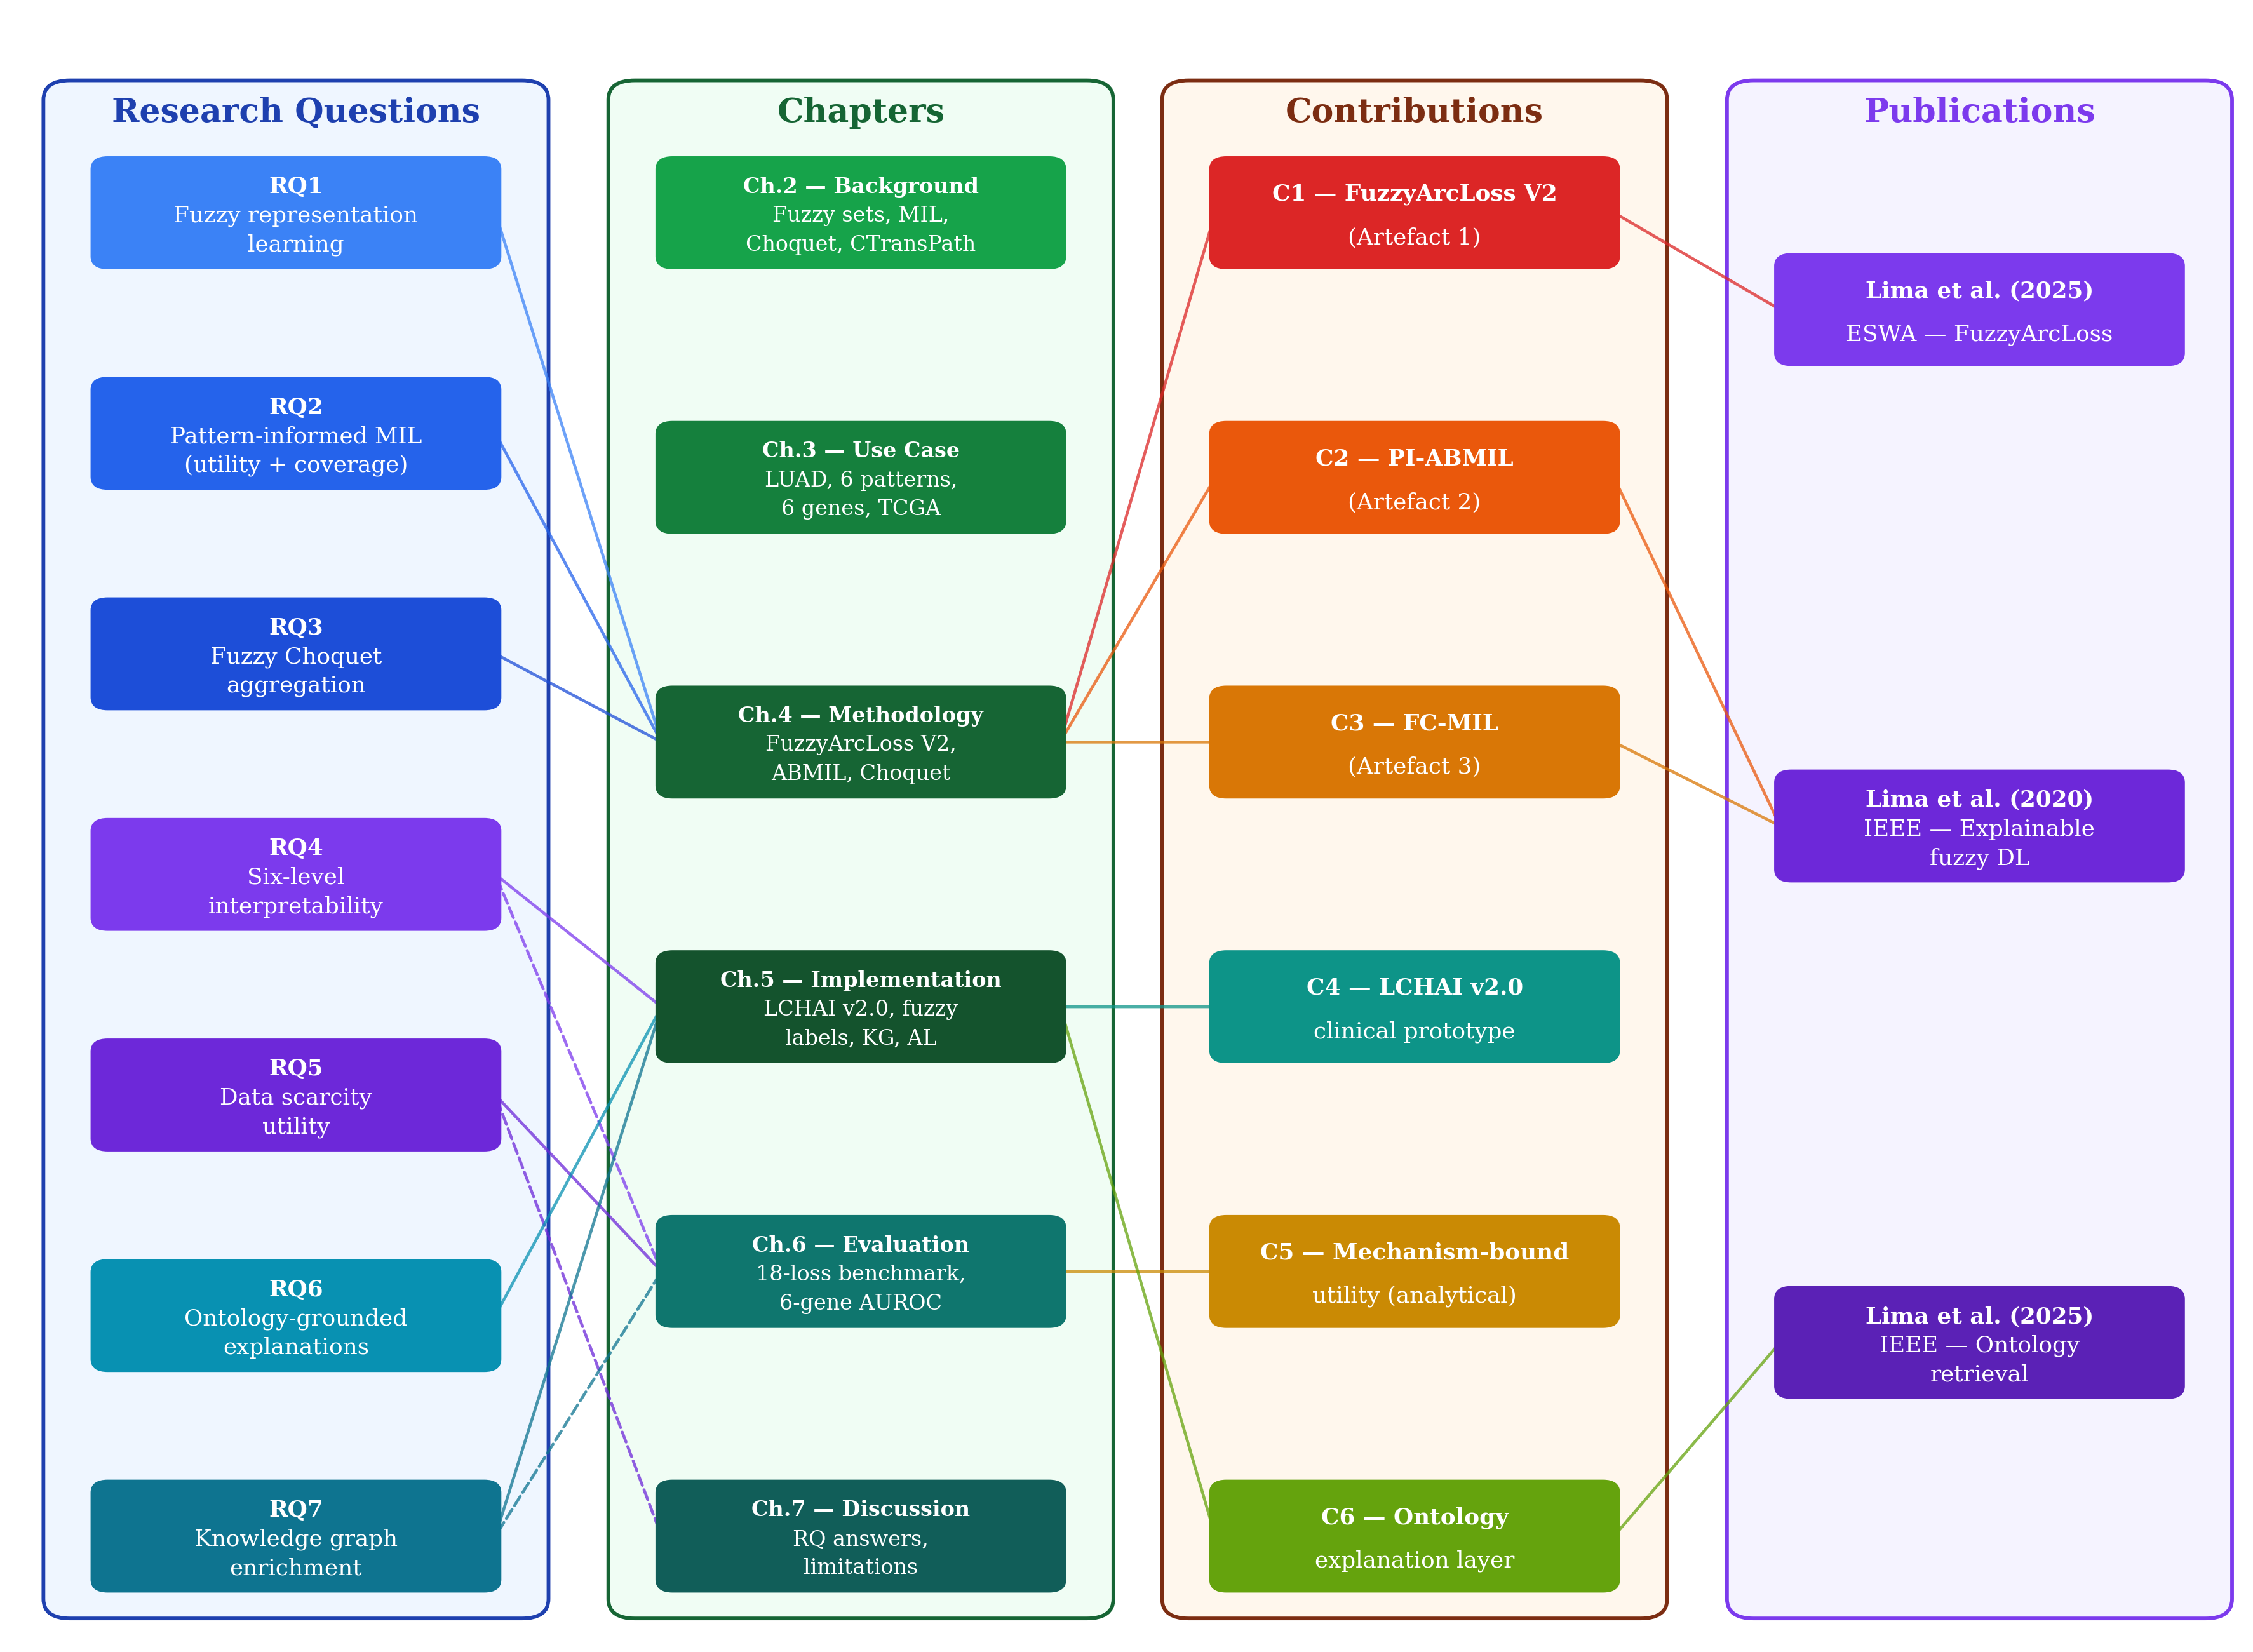
\includegraphics[width=\textwidth]{chapters/figures/thesis_visual_summary.png}
\caption[Visual summary of the thesis]{%
    Visual summary of the thesis.
    \textbf{Left}: Seven research questions (RQ1--RQ7) framed from a
    computer science perspective.
    \textbf{Centre}: Six thesis chapters where each RQ is addressed.
    \textbf{Right-centre}: Six contributions produced by the thesis.
    \textbf{Far right}: Three prior publications by the author, each
    extended in this work.
    Solid arrows indicate the primary mapping between questions,
    chapters, contributions, and publications; dashed arrows mark
    secondary anchorings that span more than one chapter.}
\label{fig:thesis_visual_summary}
\end{figure}


% ============================================================
\section{Contributions}
\label{sec:intro:contributions}
% ============================================================

The principal contributions of this thesis are:

\begin{enumerate}
    \item \textbf{C1 --- FuzzyArcLoss~V2 (Artefact 1).}
    A novel angular margin loss function that adapts the angular
    penalty per-sample through an explicit fuzzy membership function
    $\mu$, reducing the margin for ambiguous samples near class
    boundaries.
    The method is targeted at histopathological pattern classification,
    where inter-class transitions are inherently fuzzy.
    Specified in Chapter~\ref{ch:methodology}, evaluated against
    fixed-margin baselines in Chapter~\ref{ch:evaluation}, and
    discussed in Chapter~\ref{ch:discussion}.

    \item \textbf{C2 --- Pattern-informed ABMIL (Artefact 2).}
    The first attention-based MIL architecture to concatenate
    validated fuzzy histological pattern probabilities with
    self-supervised visual embeddings as input to a mutation
    prediction aggregator, enabling a six-level interpretability
    framework over the same trained model.
    Designed in Chapter~\ref{ch:methodology}, implemented in
    Chapter~\ref{ch:implementation}, evaluated in
    Chapter~\ref{ch:evaluation}, and discussed in
    Chapter~\ref{ch:discussion}.

    \item \textbf{C3 --- Fuzzy Choquet MIL (Artefact 3).}
    A novel MIL aggregation module based on the discrete Choquet
    integral with a learned 2-additive fuzzy measure, designed to
    capture supra-additive interactions between histological patterns
    and to expose them as interpretable Shapley values and pairwise
    interaction indices.
    Specified in Chapter~\ref{ch:methodology}, evaluated against
    attention-based aggregation in Chapter~\ref{ch:evaluation}, and
    discussed in Chapter~\ref{ch:discussion}.

    \item \textbf{C4 --- LCHAI~v2.0 clinical prototype.}
    An integrative clinical decision-support system that demonstrates
    the translational potential of artefacts C1--C3 within a unified
    workflow on TCGA-LUAD~\cite{tcga2014luad}, combining tile-level
    pattern classification, slide-level mutation prediction with
    confidence calibration, the six-level interpretability framework
    of C2, and a biomedical knowledge graph linking mutations to
    therapeutic targets.
    Implemented in Chapter~\ref{ch:implementation}, evaluated through
    a multi-condition cross-validated benchmark in
    Chapter~\ref{ch:evaluation}, and discussed in
    Chapter~\ref{ch:discussion}.

    \item \textbf{C5 --- Mechanism-bound utility of fuzzy
    representations (analytical insight).}
    An analytical contribution that characterises \emph{when} fuzzy
    pattern encodings provide a measurable advantage over crisp
    one-hot encodings in mutation prediction, framed in terms of the
    aggregator's ability to model inter-pattern interactions rather
    than as a property of any specific gene set.
    Established through the per-gene and per-slide ablation analyses
    of Chapter~\ref{ch:evaluation} and synthesised in
    Chapter~\ref{ch:discussion}.

    \item \textbf{C6 --- Ontology-grounded explanation layer.}
    A three-tier knowledge graph architecture---a curated layer of
    clinical assertions, a dynamic per-case filtering layer, and a
    DeepSearch literature enrichment layer---that links predicted
    mutations to therapeutic targets through provenance-tagged
    relations grounded in NCIt and MONDO ontologies (RQ6, RQ7).
    Designed in Chapter~\ref{ch:methodology}, implemented in
    Chapter~\ref{ch:implementation}, and evaluated in
    Chapter~\ref{ch:evaluation}.
\end{enumerate}


\section{Thesis as a Continuation of Prior Work}
\label{sec:continuation_prior_work}

The research findings of this dissertation have been articulated in
the following peer-reviewed publications by the author.
Each publication contributes a foundational component to the
LCHAI~v2.0 artefact developed in this thesis.

\subsection*{Journal Publication}

\begin{quote}
\textbf{Servio F.\ Lima}, Edy Portmann, and Luis Ter\'{a}n.
\emph{FuzzyArcLoss: Dynamic margin adjustment for robust recognition
across domains.}
Expert Systems with Applications, 281:127477, 2025.
DOI: \url{https://doi.org/10.1016/j.eswa.2025.127477}
\end{quote}

\begin{itemize}
    \item \textbf{Quality indicators:} Journal H-Index: 214.
    Impact Factor: 7.5 (2024). CiteScore: 13.8.
    Ranked Q1 in Computer Science Applications (12/232, 95th percentile)
    and Q1 in Engineering (11/305, 96th percentile) on SCImago.
    \item \textbf{Core contribution:} FuzzyArcLoss---a dynamic,
    sample-wise angular margin modulation mechanism for robust
    recognition under intra-class ambiguity across multiple domains.
    \item \textbf{Extension in this thesis:} FuzzyArcLoss~V2 with
    piecewise membership function, Optuna-based hyperparameter
    optimisation, and 4-channel mask input; applied to 6-class LUAD
    histological pattern classification (Artefact~1,
    Chapter~\ref{ch:methodology}).
\end{itemize}

\subsection*{Conference Publications}

\begin{quote}
\textbf{Servio F.\ Lima}, Edy Portmann, and Luis Ter\'{a}n.
\emph{A proposal for an explainable fuzzy-based deep learning system
for skin cancer prediction.}
In 2020 7th International Conference on eDemocracy \& eGovernment
(ICEDEG), pages 29--35. IEEE, 2020.
DOI: \url{https://doi.org/10.1109/ICEDEG48599.2020.9096799}
\end{quote}

\begin{itemize}
    \item \textbf{Quality indicators:} IEEE indexed.
    ICEDEG is an international conference on digital government and
    e-democracy with proceedings indexed by IEEE Xplore, Scopus,
    and Web of Science.
    \item \textbf{Core contribution:} Established the design logic of
    combining fuzzy supervision with post-hoc explanation as
    first-class requirements for clinical AI artefacts.
    \item \textbf{Extension in this thesis:} Re-instantiated from skin
    to lung pathology; dual interpretability framework (spatial
    attention maps + pattern attribution); Choquet integral as intrinsic
    explainer with Shapley values (Artefacts~2 and~3).
\end{itemize}

\begin{quote}
\textbf{Servio F.\ Lima}, Edy Portmann, and Luis Ter\'{a}n.
\emph{Enhancing cancer ontology-based query retrieval with transformer
models and adaptive angular loss functions.}
In 2025 12th International Conference on eDemocracy \& eGovernment
(ICEDEG). IEEE, 2025.
DOI: \url{https://doi.org/10.1109/ICEDEG65568.2025.11081564}
\end{quote}

\begin{itemize}
    \item \textbf{Quality indicators:} IEEE indexed.
    Proceedings indexed by IEEE Xplore, Scopus, and Web of Science.
    \item \textbf{Core contribution:} Combined transformer
    representations with adaptive angular-margin objectives for cancer
    ontology-grounded retrieval, demonstrating that geometry-shaping
    losses improve alignment between visual representations and
    structured biomedical knowledge.
    \item \textbf{Extension in this thesis:} Extended from retrieval
    to mutation prediction; knowledge graph links predicted mutations
    to therapeutic targets with PMID provenance tags
    (RQ6, RQ7, Chapter~\ref{ch:implementation}).
\end{itemize}

Together, these three publications form a research trajectory from
domain-general fuzzy representation learning, through explainable
clinical AI design, to the integrated LCHAI~v2.0 prototype.
Table~\ref{tab:prior_work_extensions} summarises the extensions.
The artefact and all experimental scripts are publicly available at
\url{https://github.com/slima2/lchai}~\cite{lchai_repo}.

\begin{table}[ht!]
\centering
\small
\caption{Prior publications by the author and their extensions in this
thesis.}
\label{tab:prior_work_extensions}
\begin{tabular}{p{3.8cm} p{3.5cm} p{5.5cm}}
\hline
\textbf{Prior work} & \textbf{Core contribution} &
\textbf{Extension in this thesis} \\
\hline
Lima et al.\ (2025) ESWA~\cite{lima2025fuzzy} &
  FuzzyArcLoss: dynamic margin modulation &
  V2 with piecewise membership, 4-channel mask, Optuna search;
  applied to 6-class LUAD pattern classification \\
Lima et al.\ (2020) IEEE~\cite{lima2020skin} &
  Explainable fuzzy DL for skin cancer &
  Re-instantiated for LUAD; dual interpretability (attention + pattern
  overlay); Choquet integral as intrinsic explainer \\
Lima et al.\ (2025) IEEE~\cite{lima2025enhancing} &
  Ontology-based retrieval with angular loss &
  Extended to mutation prediction; knowledge graph links mutations to
  pathways and treatments with provenance tags (RQ6, RQ7) \\
\hline
\end{tabular}
\end{table}
% ============================================================

% ============================================================


% ============================================================
\section{Thesis Outline}
\label{sec:intro:outline}
% ============================================================

The remainder of this thesis is organised as follows:

\begin{description}
    \item[\cref{ch:background} --- Background.]  Presents the theoretical foundations underpinning the subsequent chapters: fuzzy sets and fuzzy logic, angular margin loss functions, self-supervised learning for pathology (CTransPath), multiple-instance learning, the Choquet integral and related aggregation operators.

    \item[\cref{ch:usecase} --- The Lung Adenocarcinoma Use Case.]  Introduces the medical use case: LUAD histology, the six growth patterns (five WHO-defined plus cribriform), oncogenic driver mutations, the TCGA--LUAD dataset and the evaluation protocol.  A glossary of clinical and ML terms is provided in \cref{app:glossary}.

    \item[\cref{ch:methodology} --- Artefact Design: Conceptual Framework.]  Specifies the three artefacts at the mathematical and architectural level: FuzzyArcLoss V2 (loss function design), pattern-informed ABMIL (feature fusion architecture) and Fuzzy Choquet MIL (aggregation module).  Also presents the multi-ontology knowledge graph and explanation layer design (RQ6, RQ7).

    \item[\cref{ch:implementation} --- Implementation.]  Describes the prototypical implementation of all artefacts, including the training pipeline, hyperparameter optimisation with Optuna, embedding extraction, the ABMIL benchmark framework, the ontology-grounded explanation layer, and the LCHAI~v2.0 clinical decision-support prototype deployed on AWS EKS.

    \item[\cref{ch:evaluation} --- Evaluation.]  Reports all experimental results: the 18-loss pattern classification benchmark, the K-fold mutation prediction benchmark (6 conditions $\times$ 6 genes $\times$ 5 folds), ablation studies, statistical significance tests, comparison with the published literature, interpretability analysis with LCHAI~v2.0 pattern overlays and ABMIL attention maps for six representative slides, SHAP decomposition and Choquet Shapley value analysis, and demonstration of the knowledge graph (RQ6) and DeepSearch enrichment pipeline (RQ7).

    \item[\cref{ch:discussion} --- Discussion and Conclusion.]
    Interprets the findings in light of the research questions,
    discusses the interpretability--performance trade-off, analyses
    gene-specific behaviour and contextualises the results against
    large-scale studies (DeepGEM, EAGLE, CHIEF, GigaPath).
    Summarises the answers to each research question, identifies
    remaining limitations, and outlines future work including external
    validation, clinical deployment and extension to other cancer types.
\end{description}